\subsection{Communication Protocols and OSI Model Layers}

In designing the embedded system, several communication protocols were implemented 
to interface with various sensors and peripherals. Understanding how these protocols 
map onto the OSI model layers, particularly the physical and data link layers, is 
crucial for ensuring reliable and efficient data transmission. This section explains 
the OSI model implementation for each protocol used: SDI-12/UART/RS485, SPI, I2C, 
and analog inputs and outputs.

\subsubsection{SDI-12/UART/RS485 Communication}

\textbf{Physical Layer}

SDI-12 communication is managed using UART1 on the RP2040 microcontroller, with specific 
GPIO pins defined for transmission (TX on GPIO 8), reception (RX on GPIO 9), and data 
line drive enablement (GPIO 15). The SDI-12 protocol operates over a single data line 
with negative logic levels, where a logic '0' is represented by a voltage high, and a 
logic '1' by a voltage low. The RS485 transceiver adapts the UART signals to meet these requirements.

The RS485 transceiver is suitable for this application due to its robust communication capabilities:

\begin{itemize}
    \item Noise Immunity: RS485 uses differential signaling, enhancing noise immunity and allowing 
    reliable communication over long distances, which is essential in environmental monitoring setups.
    \item Line Driving Capability: It can drive long cables with high capacitance, ensuring signal 
    integrity between the microcontroller and sensors.
    \item Inverted Logic Handling: The transceiver accommodates the inverted logic levels required by SDI-12 devices.
\end{itemize}

By using only the non-inverting line of the RS485 transceiver and setting appropriate voltage references, 
the system effectively adapts the standard UART interface to meet the physical layer requirements of the SDI-12 protocol.

\textbf{Data Link Layer}

At the data link layer, the SDI-12 protocol defines the communication between the data recorder 
(master) and the sensors (slaves). It operates at 1200 baud with 7 data bits, even parity, and one 
stop bit. The protocol specifies a set of ASCII commands for initiating measurements, requesting 
data, and managing sensor addresses.

In the current implementation, the system communicates with two SDI-12 sensors whose addresses are 
hardcoded. This approach simplifies the software but limits the system's scalability and flexibility. 
SDI-12 allows for up to ten sensors on a single data line, each with a unique address. A more extensible 
system would implement a discovery process using the SDI-12 "Address Query" command (?!) to identify 
all connected sensors dynamically. This would enable the system to communicate with any number of sensors 
without prior knowledge of their addresses, fully utilizing the hardware's capability for extensibility.

\textbf{Application Layer}

Custom drivers were developed for each sensor, adhering to the SDI-12 
protocol. Specific issues with the byte framing of the SDI-12 protocol were addressed by using the 
\code{uart_set_format()} function to configure the communication format correctly, allowing the RP2040 
to receive the inverted data without additional circuitry. The \code{uart_break()} function was used to 
send the break signal while the \code{uart_read_stuff()} function was used to read the response from 
the sensor. The response was then parsed to get the data. The timing of the SDI-12 protocol is shown 
in \cref{sdi12_timing}.

\begin{figure}
    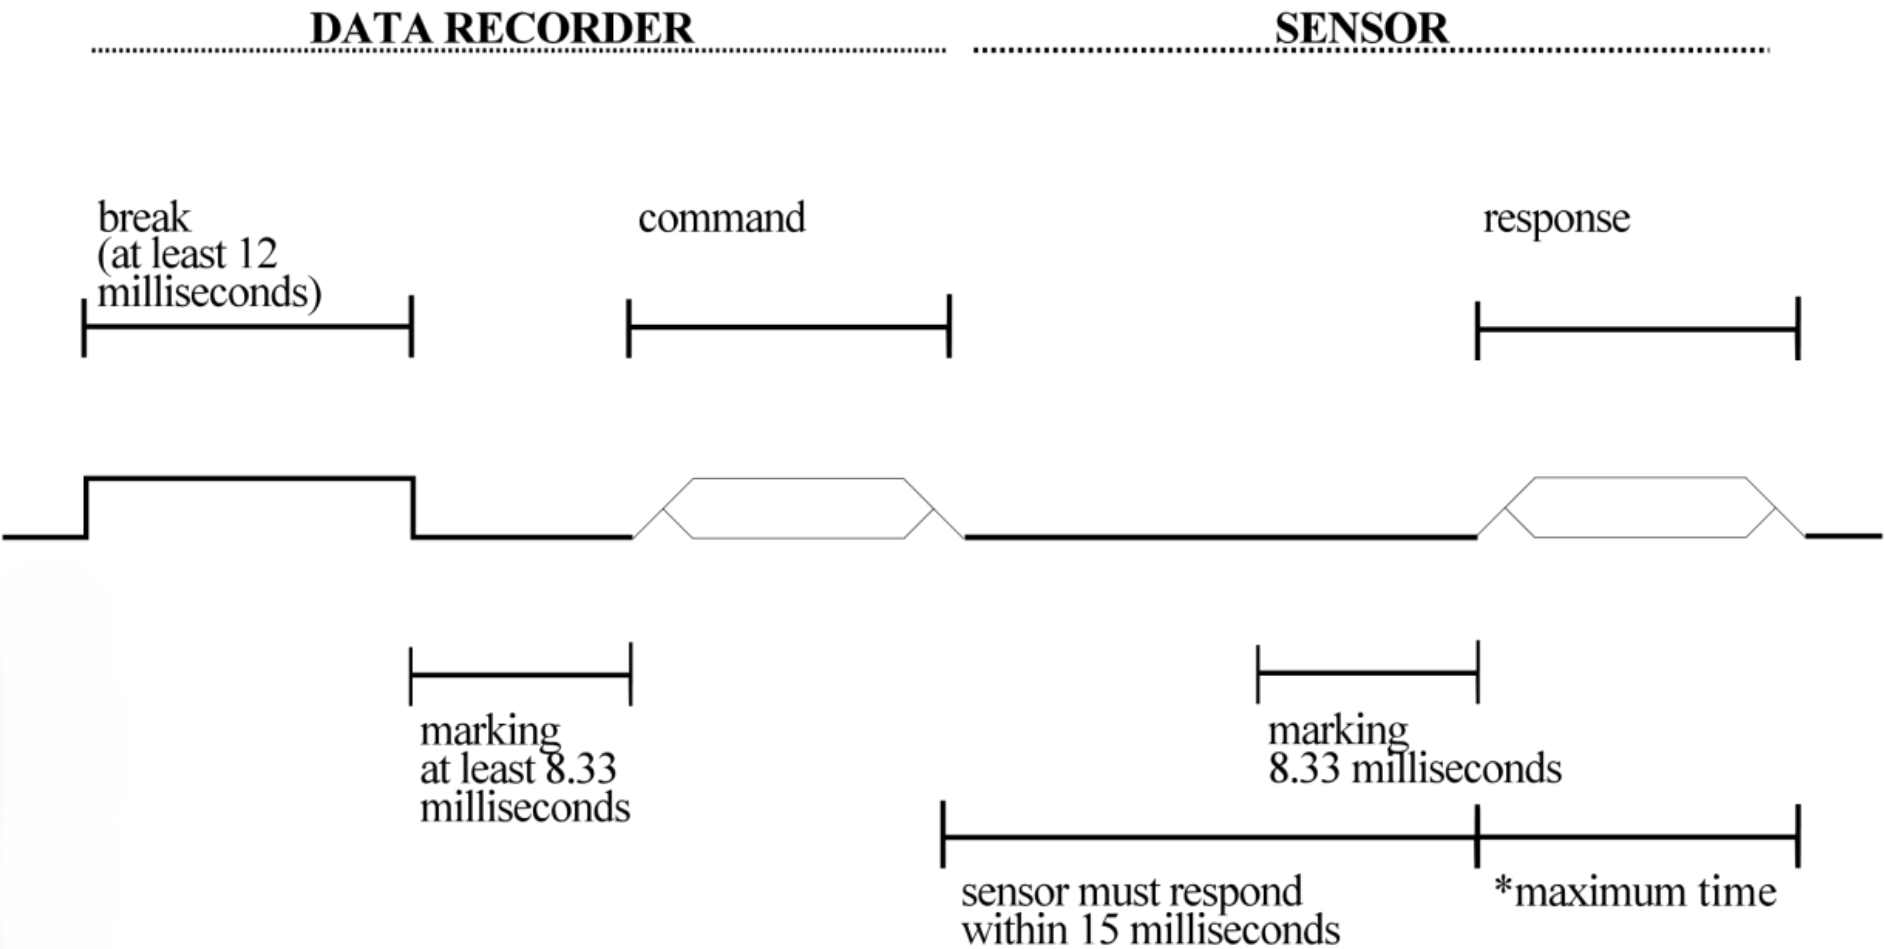
\includegraphics[width=\linewidth]{figures/SDI-12_timing.png}
    \caption{SDI-12 timing from \cite{sdi12_datasheet}}
    \label{sdi12_timing}
\end{figure}

\subsubsection{SPI Communication (SD Card)}

\textbf{Physical Layer}

The SPI protocol is used for communication with the SD card module. SPI is a synchronous serial communication 
interface that operates in full-duplex mode. It uses four signals:
\begin{itemize}
    \item MOSI (Master Out Slave In): Transfers data from the master to the slave.
    \item MISO (Master In Slave Out): Transfers data from the slave to the master.
    \item SCK (Serial Clock): Synchronises data transmission between the master and slave.
    \item SS (Slave Select): Enables the slave device for communication.
\end{itemize}
In this system, the SPI bus operates at a clock speed of 1 MHz, suitable for reliable data transfer 
with the SD card.

\textbf{Data Link Layer}

At the data link layer, the SPI protocol manages the exchange of data bytes between the microcontroller 
and the SD card. It does not define a specific frame format or error-checking mechanism, relying on 
higher-level protocols for these functions. The FatFs file system library is employed to handle file 
operations on the SD card. FatFs provides functions for reading, writing, and managing files, ensuring 
data integrity and proper formatting according to the FAT file system standards.

\textbf{Application Layer}

The FatFs API was integrated to enable read/write operations on the SD card, 
using the SPI protocol. This allowed for structured data logging and easy retrieval of information. 
Functions were implemented to write data in CSV format, facilitating compatibility with data analysis tools.

\subsubsection{I2C Communication (DAC)}

\textbf{Physical Layer}

The I2C protocol is used for communication with the MCP4716 DAC. I2C is a synchronous, multi-master, 
multi-slave, single-ended serial communication bus. It uses two bidirectional open-drain lines:
\begin{itemize}
    \item SDA (Serial Data Line): Transfers data between devices.
    \item SCL (Serial Clock Line): Provides the clock signal for synchronisation.
\end{itemize}
Pull-up resistors are used on both lines to maintain the high logic level when the bus is idle. 
In this system, the I2C bus operates at a standard mode speed of 100 kHz.

\textbf{Data Link Layer}

At the data link layer, the I2C protocol handles addressing and data transfer between the master 
(RP2040 microcontroller) and the slave device (DAC). Each device on the I2C bus has a unique 7-bit address. 
The protocol defines start and stop conditions, acknowledgments, and data byte transfers. The software includes drivers to configure the DAC's settings, such as reference voltage and gain, and to send digital values that the DAC converts into analog voltages. This allows precise control over the dew point generator.

\subsubsection{Analogue Inputs and Outputs}

\textbf{Physical Layer}

Analog inputs and outputs are used to interface with devices like the load cell (MT-603) and the dew point 
generator (LI-610). The load cell produces an analog voltage proportional to the applied weight, which is 
connected to the RP2040's ADC pins. An instrumentation amplifier (e.g., INA826) is used to amplify the small 
signal from the load cell. The dew point generator accepts a 0–5 V analog input for control, which is 
provided by the DAC's output.

\textbf{Data Link Layer}

In the context of analog signals, there is no formal data link layer as in digital communication protocols. 
However, signal conditioning and conversion processes serve similar functions. For analog inputs, the signal 
from the load cell is amplified and filtered before being digitized by the ADC. For analog outputs, the DAC 
converts digital values from the microcontroller into precise analog voltages to control the dew point 
generator's settings.

\textbf{Application Layer}

A software interface for controlling the dew point generator was implemented 
using the I2C protocol to communicate with the DAC. This interface allows precise voltage adjustments to 
the generator, with preliminary tests confirming accurate output predictions based on command inputs. 
The I2C communication was established using standard mode at 100 kHz, which is compatible with the MCP4716 DAC.

The careful selection of communication interfaces and voltage levels, along with robust software 
integration, allowed the system to operate seamlessly and efficiently, providing a reliable solution 
for monitoring and controlling environmental parameters.

